\documentclass{article} % For LaTeX2e
\usepackage[T1]{fontenc}
\usepackage{iclr2025_conference,times}

%%%%% NEW MATH DEFINITIONS %%%%%

\usepackage{amsmath,amsfonts,bm}

% Mark sections of captions for referring to divisions of figures
\newcommand{\figleft}{{\em (Left)}}
\newcommand{\figcenter}{{\em (Center)}}
\newcommand{\figright}{{\em (Right)}}
\newcommand{\figtop}{{\em (Top)}}
\newcommand{\figbottom}{{\em (Bottom)}}
\newcommand{\captiona}{{\em (a)}}
\newcommand{\captionb}{{\em (b)}}
\newcommand{\captionc}{{\em (c)}}
\newcommand{\captiond}{{\em (d)}}

% Highlight a newly defined term
\newcommand{\newterm}[1]{{\bf #1}}


% Figure reference, lower-case.
\def\figref#1{figure~\ref{#1}}
% Figure reference, capital. For start of sentence
\def\Figref#1{Figure~\ref{#1}}
\def\twofigref#1#2{figures \ref{#1} and \ref{#2}}
\def\quadfigref#1#2#3#4{figures \ref{#1}, \ref{#2}, \ref{#3} and \ref{#4}}
% Section reference, lower-case.
\def\secref#1{section~\ref{#1}}
% Section reference, capital.
\def\Secref#1{Section~\ref{#1}}
% Reference to two sections.
\def\twosecrefs#1#2{sections \ref{#1} and \ref{#2}}
% Reference to three sections.
\def\secrefs#1#2#3{sections \ref{#1}, \ref{#2} and \ref{#3}}
% Reference to an equation, lower-case.
\def\eqref#1{equation~\ref{#1}}
% Reference to an equation, upper case
\def\Eqref#1{Equation~\ref{#1}}
% A raw reference to an equation---avoid using if possible
\def\plaineqref#1{\ref{#1}}
% Reference to a chapter, lower-case.
\def\chapref#1{chapter~\ref{#1}}
% Reference to an equation, upper case.
\def\Chapref#1{Chapter~\ref{#1}}
% Reference to a range of chapters
\def\rangechapref#1#2{chapters\ref{#1}--\ref{#2}}
% Reference to an algorithm, lower-case.
\def\algref#1{algorithm~\ref{#1}}
% Reference to an algorithm, upper case.
\def\Algref#1{Algorithm~\ref{#1}}
\def\twoalgref#1#2{algorithms \ref{#1} and \ref{#2}}
\def\Twoalgref#1#2{Algorithms \ref{#1} and \ref{#2}}
% Reference to a part, lower case
\def\partref#1{part~\ref{#1}}
% Reference to a part, upper case
\def\Partref#1{Part~\ref{#1}}
\def\twopartref#1#2{parts \ref{#1} and \ref{#2}}

\def\ceil#1{\lceil #1 \rceil}
\def\floor#1{\lfloor #1 \rfloor}
\def\1{\bm{1}}
\newcommand{\train}{\mathcal{D}}
\newcommand{\valid}{\mathcal{D_{\mathrm{valid}}}}
\newcommand{\test}{\mathcal{D_{\mathrm{test}}}}

\def\eps{{\epsilon}}


% Random variables
\def\reta{{\textnormal{$\eta$}}}
\def\ra{{\textnormal{a}}}
\def\rb{{\textnormal{b}}}
\def\rc{{\textnormal{c}}}
\def\rd{{\textnormal{d}}}
\def\re{{\textnormal{e}}}
\def\rf{{\textnormal{f}}}
\def\rg{{\textnormal{g}}}
\def\rh{{\textnormal{h}}}
\def\ri{{\textnormal{i}}}
\def\rj{{\textnormal{j}}}
\def\rk{{\textnormal{k}}}
\def\rl{{\textnormal{l}}}
% rm is already a command, just don't name any random variables m
\def\rn{{\textnormal{n}}}
\def\ro{{\textnormal{o}}}
\def\rp{{\textnormal{p}}}
\def\rq{{\textnormal{q}}}
\def\rr{{\textnormal{r}}}
\def\rs{{\textnormal{s}}}
\def\rt{{\textnormal{t}}}
\def\ru{{\textnormal{u}}}
\def\rv{{\textnormal{v}}}
\def\rw{{\textnormal{w}}}
\def\rx{{\textnormal{x}}}
\def\ry{{\textnormal{y}}}
\def\rz{{\textnormal{z}}}

% Random vectors
\def\rvepsilon{{\mathbf{\epsilon}}}
\def\rvtheta{{\mathbf{\theta}}}
\def\rva{{\mathbf{a}}}
\def\rvb{{\mathbf{b}}}
\def\rvc{{\mathbf{c}}}
\def\rvd{{\mathbf{d}}}
\def\rve{{\mathbf{e}}}
\def\rvf{{\mathbf{f}}}
\def\rvg{{\mathbf{g}}}
\def\rvh{{\mathbf{h}}}
\def\rvu{{\mathbf{i}}}
\def\rvj{{\mathbf{j}}}
\def\rvk{{\mathbf{k}}}
\def\rvl{{\mathbf{l}}}
\def\rvm{{\mathbf{m}}}
\def\rvn{{\mathbf{n}}}
\def\rvo{{\mathbf{o}}}
\def\rvp{{\mathbf{p}}}
\def\rvq{{\mathbf{q}}}
\def\rvr{{\mathbf{r}}}
\def\rvs{{\mathbf{s}}}
\def\rvt{{\mathbf{t}}}
\def\rvu{{\mathbf{u}}}
\def\rvv{{\mathbf{v}}}
\def\rvw{{\mathbf{w}}}
\def\rvx{{\mathbf{x}}}
\def\rvy{{\mathbf{y}}}
\def\rvz{{\mathbf{z}}}

% Elements of random vectors
\def\erva{{\textnormal{a}}}
\def\ervb{{\textnormal{b}}}
\def\ervc{{\textnormal{c}}}
\def\ervd{{\textnormal{d}}}
\def\erve{{\textnormal{e}}}
\def\ervf{{\textnormal{f}}}
\def\ervg{{\textnormal{g}}}
\def\ervh{{\textnormal{h}}}
\def\ervi{{\textnormal{i}}}
\def\ervj{{\textnormal{j}}}
\def\ervk{{\textnormal{k}}}
\def\ervl{{\textnormal{l}}}
\def\ervm{{\textnormal{m}}}
\def\ervn{{\textnormal{n}}}
\def\ervo{{\textnormal{o}}}
\def\ervp{{\textnormal{p}}}
\def\ervq{{\textnormal{q}}}
\def\ervr{{\textnormal{r}}}
\def\ervs{{\textnormal{s}}}
\def\ervt{{\textnormal{t}}}
\def\ervu{{\textnormal{u}}}
\def\ervv{{\textnormal{v}}}
\def\ervw{{\textnormal{w}}}
\def\ervx{{\textnormal{x}}}
\def\ervy{{\textnormal{y}}}
\def\ervz{{\textnormal{z}}}

% Random matrices
\def\rmA{{\mathbf{A}}}
\def\rmB{{\mathbf{B}}}
\def\rmC{{\mathbf{C}}}
\def\rmD{{\mathbf{D}}}
\def\rmE{{\mathbf{E}}}
\def\rmF{{\mathbf{F}}}
\def\rmG{{\mathbf{G}}}
\def\rmH{{\mathbf{H}}}
\def\rmI{{\mathbf{I}}}
\def\rmJ{{\mathbf{J}}}
\def\rmK{{\mathbf{K}}}
\def\rmL{{\mathbf{L}}}
\def\rmM{{\mathbf{M}}}
\def\rmN{{\mathbf{N}}}
\def\rmO{{\mathbf{O}}}
\def\rmP{{\mathbf{P}}}
\def\rmQ{{\mathbf{Q}}}
\def\rmR{{\mathbf{R}}}
\def\rmS{{\mathbf{S}}}
\def\rmT{{\mathbf{T}}}
\def\rmU{{\mathbf{U}}}
\def\rmV{{\mathbf{V}}}
\def\rmW{{\mathbf{W}}}
\def\rmX{{\mathbf{X}}}
\def\rmY{{\mathbf{Y}}}
\def\rmZ{{\mathbf{Z}}}

% Elements of random matrices
\def\ermA{{\textnormal{A}}}
\def\ermB{{\textnormal{B}}}
\def\ermC{{\textnormal{C}}}
\def\ermD{{\textnormal{D}}}
\def\ermE{{\textnormal{E}}}
\def\ermF{{\textnormal{F}}}
\def\ermG{{\textnormal{G}}}
\def\ermH{{\textnormal{H}}}
\def\ermI{{\textnormal{I}}}
\def\ermJ{{\textnormal{J}}}
\def\ermK{{\textnormal{K}}}
\def\ermL{{\textnormal{L}}}
\def\ermM{{\textnormal{M}}}
\def\ermN{{\textnormal{N}}}
\def\ermO{{\textnormal{O}}}
\def\ermP{{\textnormal{P}}}
\def\ermQ{{\textnormal{Q}}}
\def\ermR{{\textnormal{R}}}
\def\ermS{{\textnormal{S}}}
\def\ermT{{\textnormal{T}}}
\def\ermU{{\textnormal{U}}}
\def\ermV{{\textnormal{V}}}
\def\ermW{{\textnormal{W}}}
\def\ermX{{\textnormal{X}}}
\def\ermY{{\textnormal{Y}}}
\def\ermZ{{\textnormal{Z}}}

% Vectors
\def\vzero{{\bm{0}}}
\def\vone{{\bm{1}}}
\def\vmu{{\bm{\mu}}}
\def\vtheta{{\bm{\theta}}}
\def\va{{\bm{a}}}
\def\vb{{\bm{b}}}
\def\vc{{\bm{c}}}
\def\vd{{\bm{d}}}
\def\ve{{\bm{e}}}
\def\vf{{\bm{f}}}
\def\vg{{\bm{g}}}
\def\vh{{\bm{h}}}
\def\vi{{\bm{i}}}
\def\vj{{\bm{j}}}
\def\vk{{\bm{k}}}
\def\vl{{\bm{l}}}
\def\vm{{\bm{m}}}
\def\vn{{\bm{n}}}
\def\vo{{\bm{o}}}
\def\vp{{\bm{p}}}
\def\vq{{\bm{q}}}
\def\vr{{\bm{r}}}
\def\vs{{\bm{s}}}
\def\vt{{\bm{t}}}
\def\vu{{\bm{u}}}
\def\vv{{\bm{v}}}
\def\vw{{\bm{w}}}
\def\vx{{\bm{x}}}
\def\vy{{\bm{y}}}
\def\vz{{\bm{z}}}

% Elements of vectors
\def\evalpha{{\alpha}}
\def\evbeta{{\beta}}
\def\evepsilon{{\epsilon}}
\def\evlambda{{\lambda}}
\def\evomega{{\omega}}
\def\evmu{{\mu}}
\def\evpsi{{\psi}}
\def\evsigma{{\sigma}}
\def\evtheta{{\theta}}
\def\eva{{a}}
\def\evb{{b}}
\def\evc{{c}}
\def\evd{{d}}
\def\eve{{e}}
\def\evf{{f}}
\def\evg{{g}}
\def\evh{{h}}
\def\evi{{i}}
\def\evj{{j}}
\def\evk{{k}}
\def\evl{{l}}
\def\evm{{m}}
\def\evn{{n}}
\def\evo{{o}}
\def\evp{{p}}
\def\evq{{q}}
\def\evr{{r}}
\def\evs{{s}}
\def\evt{{t}}
\def\evu{{u}}
\def\evv{{v}}
\def\evw{{w}}
\def\evx{{x}}
\def\evy{{y}}
\def\evz{{z}}

% Matrix
\def\mA{{\bm{A}}}
\def\mB{{\bm{B}}}
\def\mC{{\bm{C}}}
\def\mD{{\bm{D}}}
\def\mE{{\bm{E}}}
\def\mF{{\bm{F}}}
\def\mG{{\bm{G}}}
\def\mH{{\bm{H}}}
\def\mI{{\bm{I}}}
\def\mJ{{\bm{J}}}
\def\mK{{\bm{K}}}
\def\mL{{\bm{L}}}
\def\mM{{\bm{M}}}
\def\mN{{\bm{N}}}
\def\mO{{\bm{O}}}
\def\mP{{\bm{P}}}
\def\mQ{{\bm{Q}}}
\def\mR{{\bm{R}}}
\def\mS{{\bm{S}}}
\def\mT{{\bm{T}}}
\def\mU{{\bm{U}}}
\def\mV{{\bm{V}}}
\def\mW{{\bm{W}}}
\def\mX{{\bm{X}}}
\def\mY{{\bm{Y}}}
\def\mZ{{\bm{Z}}}
\def\mBeta{{\bm{\beta}}}
\def\mPhi{{\bm{\Phi}}}
\def\mLambda{{\bm{\Lambda}}}
\def\mSigma{{\bm{\Sigma}}}

% Tensor
\DeclareMathAlphabet{\mathsfit}{\encodingdefault}{\sfdefault}{m}{sl}
\SetMathAlphabet{\mathsfit}{bold}{\encodingdefault}{\sfdefault}{bx}{n}
\newcommand{\tens}[1]{\bm{\mathsfit{#1}}}
\def\tA{{\tens{A}}}
\def\tB{{\tens{B}}}
\def\tC{{\tens{C}}}
\def\tD{{\tens{D}}}
\def\tE{{\tens{E}}}
\def\tF{{\tens{F}}}
\def\tG{{\tens{G}}}
\def\tH{{\tens{H}}}
\def\tI{{\tens{I}}}
\def\tJ{{\tens{J}}}
\def\tK{{\tens{K}}}
\def\tL{{\tens{L}}}
\def\tM{{\tens{M}}}
\def\tN{{\tens{N}}}
\def\tO{{\tens{O}}}
\def\tP{{\tens{P}}}
\def\tQ{{\tens{Q}}}
\def\tR{{\tens{R}}}
\def\tS{{\tens{S}}}
\def\tT{{\tens{T}}}
\def\tU{{\tens{U}}}
\def\tV{{\tens{V}}}
\def\tW{{\tens{W}}}
\def\tX{{\tens{X}}}
\def\tY{{\tens{Y}}}
\def\tZ{{\tens{Z}}}


% Graph
\def\gA{{\mathcal{A}}}
\def\gB{{\mathcal{B}}}
\def\gC{{\mathcal{C}}}
\def\gD{{\mathcal{D}}}
\def\gE{{\mathcal{E}}}
\def\gF{{\mathcal{F}}}
\def\gG{{\mathcal{G}}}
\def\gH{{\mathcal{H}}}
\def\gI{{\mathcal{I}}}
\def\gJ{{\mathcal{J}}}
\def\gK{{\mathcal{K}}}
\def\gL{{\mathcal{L}}}
\def\gM{{\mathcal{M}}}
\def\gN{{\mathcal{N}}}
\def\gO{{\mathcal{O}}}
\def\gP{{\mathcal{P}}}
\def\gQ{{\mathcal{Q}}}
\def\gR{{\mathcal{R}}}
\def\gS{{\mathcal{S}}}
\def\gT{{\mathcal{T}}}
\def\gU{{\mathcal{U}}}
\def\gV{{\mathcal{V}}}
\def\gW{{\mathcal{W}}}
\def\gX{{\mathcal{X}}}
\def\gY{{\mathcal{Y}}}
\def\gZ{{\mathcal{Z}}}

% Sets
\def\sA{{\mathbb{A}}}
\def\sB{{\mathbb{B}}}
\def\sC{{\mathbb{C}}}
\def\sD{{\mathbb{D}}}
% Don't use a set called E, because this would be the same as our symbol
% for expectation.
\def\sF{{\mathbb{F}}}
\def\sG{{\mathbb{G}}}
\def\sH{{\mathbb{H}}}
\def\sI{{\mathbb{I}}}
\def\sJ{{\mathbb{J}}}
\def\sK{{\mathbb{K}}}
\def\sL{{\mathbb{L}}}
\def\sM{{\mathbb{M}}}
\def\sN{{\mathbb{N}}}
\def\sO{{\mathbb{O}}}
\def\sP{{\mathbb{P}}}
\def\sQ{{\mathbb{Q}}}
\def\sR{{\mathbb{R}}}
\def\sS{{\mathbb{S}}}
\def\sT{{\mathbb{T}}}
\def\sU{{\mathbb{U}}}
\def\sV{{\mathbb{V}}}
\def\sW{{\mathbb{W}}}
\def\sX{{\mathbb{X}}}
\def\sY{{\mathbb{Y}}}
\def\sZ{{\mathbb{Z}}}

% Entries of a matrix
\def\emLambda{{\Lambda}}
\def\emA{{A}}
\def\emB{{B}}
\def\emC{{C}}
\def\emD{{D}}
\def\emE{{E}}
\def\emF{{F}}
\def\emG{{G}}
\def\emH{{H}}
\def\emI{{I}}
\def\emJ{{J}}
\def\emK{{K}}
\def\emL{{L}}
\def\emM{{M}}
\def\emN{{N}}
\def\emO{{O}}
\def\emP{{P}}
\def\emQ{{Q}}
\def\emR{{R}}
\def\emS{{S}}
\def\emT{{T}}
\def\emU{{U}}
\def\emV{{V}}
\def\emW{{W}}
\def\emX{{X}}
\def\emY{{Y}}
\def\emZ{{Z}}
\def\emSigma{{\Sigma}}

% entries of a tensor
% Same font as tensor, without \bm wrapper
\newcommand{\etens}[1]{\mathsfit{#1}}
\def\etLambda{{\etens{\Lambda}}}
\def\etA{{\etens{A}}}
\def\etB{{\etens{B}}}
\def\etC{{\etens{C}}}
\def\etD{{\etens{D}}}
\def\etE{{\etens{E}}}
\def\etF{{\etens{F}}}
\def\etG{{\etens{G}}}
\def\etH{{\etens{H}}}
\def\etI{{\etens{I}}}
\def\etJ{{\etens{J}}}
\def\etK{{\etens{K}}}
\def\etL{{\etens{L}}}
\def\etM{{\etens{M}}}
\def\etN{{\etens{N}}}
\def\etO{{\etens{O}}}
\def\etP{{\etens{P}}}
\def\etQ{{\etens{Q}}}
\def\etR{{\etens{R}}}
\def\etS{{\etens{S}}}
\def\etT{{\etens{T}}}
\def\etU{{\etens{U}}}
\def\etV{{\etens{V}}}
\def\etW{{\etens{W}}}
\def\etX{{\etens{X}}}
\def\etY{{\etens{Y}}}
\def\etZ{{\etens{Z}}}

% The true underlying data generating distribution
\newcommand{\pdata}{p_{\rm{data}}}
% The empirical distribution defined by the training set
\newcommand{\ptrain}{\hat{p}_{\rm{data}}}
\newcommand{\Ptrain}{\hat{P}_{\rm{data}}}
% The model distribution
\newcommand{\pmodel}{p_{\rm{model}}}
\newcommand{\Pmodel}{P_{\rm{model}}}
\newcommand{\ptildemodel}{\tilde{p}_{\rm{model}}}
% Stochastic autoencoder distributions
\newcommand{\pencode}{p_{\rm{encoder}}}
\newcommand{\pdecode}{p_{\rm{decoder}}}
\newcommand{\precons}{p_{\rm{reconstruct}}}

\newcommand{\laplace}{\mathrm{Laplace}} % Laplace distribution

\newcommand{\E}{\mathbb{E}}
\newcommand{\Ls}{\mathcal{L}}
\newcommand{\R}{\mathbb{R}}
\newcommand{\emp}{\tilde{p}}
\newcommand{\lr}{\alpha}
\newcommand{\reg}{\lambda}
\newcommand{\rect}{\mathrm{rectifier}}
\newcommand{\softmax}{\mathrm{softmax}}
\newcommand{\sigmoid}{\sigma}
\newcommand{\softplus}{\zeta}
\newcommand{\KL}{D_{\mathrm{KL}}}
\newcommand{\Var}{\mathrm{Var}}
\newcommand{\standarderror}{\mathrm{SE}}
\newcommand{\Cov}{\mathrm{Cov}}
% Wolfram Mathworld says $L^2$ is for function spaces and $\ell^2$ is for vectors
% But then they seem to use $L^2$ for vectors throughout the site, and so does
% wikipedia.
\newcommand{\normlzero}{L^0}
\newcommand{\normlone}{L^1}
\newcommand{\normltwo}{L^2}
\newcommand{\normlp}{L^p}
\newcommand{\normmax}{L^\infty}

\newcommand{\parents}{Pa} % See usage in notation.tex. Chosen to match Daphne's book.

\DeclareMathOperator*{\argmax}{arg\,max}
\DeclareMathOperator*{\argmin}{arg\,min}

\DeclareMathOperator{\sign}{sign}
\DeclareMathOperator{\Tr}{Tr}
\let\ab\allowbreak


\usepackage{hyperref}
\usepackage{url}
\usepackage{graphicx}
\usepackage{booktabs}
\usepackage{amsmath,amssymb}
\usepackage{multirow}
\usepackage{xcolor}
\usepackage{enumitem}
\setlist{itemsep=0.1em,topsep=0.25em}

\newcommand{\an}[1]{\texttt{#1}}
\newcommand{\run}[1]{\texttt{#1}}

\title{Orvessa: How Far Does a Small LLM\\ Learn a Language It Has Never Seen?}

\author{Kavinraj \\
Group 14, roll number 24IM10055 \\
Indian Institute of Technology Kharagpur \\
Course project, AI60213 Foundations of Large Language Models \\
Code: \url{https://github.com/Lsidvd234/alien-rosetta}
}

\iclrfinalcopy
\begin{document}

\maketitle
\lhead{}\renewcommand{\headrulewidth}{0pt}

\begin{abstract}
Studying how a language model learns a new language is hard with real languages: the model may have seen them in
pretraining, and there is no exact answer key. We build a generator that invents a complete Tamil-like language
(subject--object--verb order, case and agreement endings, sound changes, 11,078 root words) written in 27 invented
glyphs that no tokenizer has seen, with a deterministic translation for every English sentence. We fine-tune
Qwen3-0.6B-Base with LoRA to translate English into it, first writing a structured \emph{meaning analysis} and then
the glyphs, so every error can be split into a misreading of the English or a mistake in the new language. Across
165 training runs on free GPUs we find: (A) generalisation stops at what training covers: held-out English
structures score 0.00--0.09, while putting back only 50 passive sentences (0.06\% of the data) lifts passive
reading from 0.00 to 0.53--0.66; (B) a spelling rule transfers to never-seen words when it covers the whole vocabulary
(0.67) but is learned mostly as a list when it covers a 4--12\% minority (0.19--0.27); (C) on real English only more
varied English helps (Tatoeba meaning 0.62 $\rightarrow$ 0.92, 2 seeds), while focal loss, paraphrases, more epochs,
decoding tricks and a 3$\times$ larger model do not; (D) on real English the failures are in \emph{reading} the
English, and where the English has words the training never had, in both reading and writing; probes and steering
show that the output is written from the model's English meaning representation, where most errors already sit;
(E) in arithmetic written in glyph digits, a fact removed from training is rebuilt only from facts the model has seen
in the same role, and five examples of that role are enough.
\end{abstract}

%=====================================================================
\section{Introduction}

Large language models are increasingly adapted to low-resource languages, new notations and domain scripts, often
with a small model and a parameter-efficient method such as LoRA \citep{hu2022lora}. What such a model can and cannot
learn from a modest amount of parallel data is therefore a practical question. It is also a hard one to answer
cleanly with real languages: pretraining may already contain the language, the gold translations are themselves
noisy, and one cannot change a single property of a real language and keep everything else fixed.

We take the opposite route and \emph{invent} the language. A generator produces a language with a fixed grammar,
vocabulary and script, renders any meaning into it deterministically, and lets us change one property at a time:
which sentence structures appear in training, which words are spelled by a rule, how much real English is mixed in.
The model has certainly never seen the language, and every test sentence has exactly one right answer. Our
research question is:

\begin{center}
\emph{What does it take for a small LLM to learn a language it has never seen, and where does that learning stop?}
\end{center}

\paragraph{Setting:} The input is an English sentence; the output is the same sentence in the invented language,
written in 27 Unicode Private Use Area glyphs, each added to the tokenizer as one new token. The main models first
write a meaning analysis such as \an{S=NAME.Tom V=beat.FUT O=PRON.2sg} and then the glyphs. Because rendering a
meaning is deterministic, any wrong output is either a \emph{reading} error (wrong analysis) or a \emph{writing}
error (right analysis, wrong glyphs). Models are tested on generated sentences, on 600 real sentences from Tatoeba
\citep{tatoeba}, and on a \emph{sealed} set of free English written by the author and frozen before it could
influence any design decision.

\paragraph{Contributions:}
\begin{itemize}
\item \textbf{A controlled testbed}: an invented-language generator with an exact answer key, a meaning-first
output that splits every error into reading vs writing, and a sealed test set used only as totals (Section~\ref{sec:setup}).
\item \textbf{Five findings with stated strength} (Section~\ref{sec:results}): (A) coverage limits structure,
with a 50-example dose that switches passives on; (B) rule vs list spelling depends on how much of the vocabulary the
rule covers; (C) only English variety helps real English, tested against eight alternatives; (D) on real English
reading fails, and with untrained words both fail, with probes and steering locating the errors in the English
representation; (E) in maths, a missing fact is rebuilt only from facts seen in the same role.
\item \textbf{Pre-registered predictions}: most extension runs had their predictions and decision rules written
before they ran, and results that missed a prediction are reported as such.
\end{itemize}

Every number states how many training runs it rests on: \emph{1 run}, \emph{2 seeds}, or a range over runs.

%=====================================================================
\section{Related work}\label{sec:related}

\textbf{Compositional and length generalisation.} Sequence models fail on held-out combinations and longer inputs
\citep{lake2018scan,kim2020cogs}, and transformers solve multi-step tasks by matching seen subgraphs rather than
composing them \citep{dziri2023faith}. Fine-tuned LLMs struggle with typologically novel features of a new
language \citep{marmonier2025explicit}, and learning a language from a grammar book is far from solved
\citep{tanzer2024mtob}. Our claim A confirms the general limit in a setting where coverage can be changed one
structure at a time and measured as a dose.

\textbf{Rules vs memorisation.} Whether a pattern is learned as a rule depends on how regular it is: the Tolerance
Principle \citep{yang2016price,schuler2016tolerance}, neural inflection models
\citep{kirov2018recurrent,mccurdy2020inflecting}, and compositional languages in neural agents
\citep{galke2024compositional}; \citet{friedman2026tolerance} find a gradual rather than sharp change in a small LM.
Claim B is a controlled same-model contrast between the two ends; we do not claim a threshold.

\textbf{Synthetic vs real input.} Semantic parsers trained on synthetic utterances fail on real ones
\citep{wang2015overnight,herzig2019detect,marzoev2020unnatural}, and scale does not close out-of-distribution gaps
\citep{qiu2022scale}. In low-resource translation the \emph{generation} side is usually the barrier
\citep{bafna2025barrier,vamvas2026romansh}; our claim D finds the opposite because here the target language is
dense in training and the English input is the unfamiliar side.

\textbf{Probing and steering.} Linear probes read features from hidden states \citep{alain2016probes}; adding
activation differences steers outputs \citep{turner2023actadd,panickssery2024caa}, including tense
\citep{klerings2025tense}; we use both as evidence for claim D, in a language learned from scratch with LoRA.
\textbf{Facts in a new role.} One stored fact does not give its reverse (the reversal curse,
\citealp{berglund2024reversal}); claim E asks when a missing fact can be rebuilt from facts the model has.

%=====================================================================
\section{Problem formulation}\label{sec:problem}

\paragraph{The language:} A generator defines a meaning space $\mathcal{M}$, an English renderer $E$ and a glyph
renderer $R$. A meaning $m\in\mathcal{M}$ is a list of events, each a set of fields (doer \an{S}, verb with tense,
aspect, modality, negation and question marks \an{V}, object \an{O}, place, manner, time, 21 relation fields, \ldots;
Appendix~\ref{app:language}). $E(m, v)$ renders $m$ as English using a surface variant $v$ (word order, voice,
contractions, casing, typos, synonyms). $R(m)$ is deterministic: it orders the words subject--object--verb, adds
case and agreement endings, applies sound changes where pieces join, and spells every sound in glyphs from the
alphabet $\Sigma$, $|\Sigma|=27$.

\paragraph{Input, process, output:} The input is an English sentence $x = E(m, v)$. The model outputs the target
string
\begin{equation}
z = m \;\Vert\; \texttt{=>} \;\Vert\; y, \qquad y = R(m),
\end{equation}
(``analysis first''), or $z=y$ for direct models. The model is a causal LM $p_\theta$ with frozen pretrained weights
$W$, LoRA updates $\Delta W = BA$ with $B\in\R^{d\times r}$, $A\in\R^{r\times d}$, $r=16$, on every attention and MLP
projection, and a trainable embedding table $E_\Sigma\in\R^{|\Sigma|\times d}$ for the new glyph tokens (tied input
and output). Training minimises the token-level cross-entropy on the target only:
\begin{equation}
\mathcal{L}(\theta) = -\sum_{(x,z)\in\mathcal{D}} \sum_{t=1}^{|z|} \log p_\theta(z_t \mid x, z_{<t}),
\qquad \theta = \{A, B, E_\Sigma\}.
\end{equation}
Each glyph $g$ spells one sound $s(g)$ (\emph{k}, \emph{zh}, \emph{aa}, \ldots); its embedding starts at the
embedding of the token for that sound, $E_\Sigma[g] \leftarrow e_{\mathrm{tok}(s(g))}$ (the sound with no letter,
the virama, starts at the mean embedding).

\paragraph{Reading and writing errors:} For a test pair $(x, m, y)$ and output $(\hat m, \hat y)$ we define
\begin{equation}
\text{reading error: } \hat m \neq m; \qquad \text{writing error: } \hat m = m \wedge \hat y \neq y .
\end{equation}
Because $R$ is deterministic, a writing error is a true error in the new language, and for a reading error we can
also check whether $\hat y = R(\hat m)$, i.e.\ the model faithfully wrote its own misreading.

\paragraph{Coverage:} For a training set $\mathcal{D}$ let $c_\mathcal{D}(k)$ count the occurrences of a meaning key
$k$ (a word, a structure feature, a multiplication fact). The questions of this paper are how accuracy on test items
depends on $c_\mathcal{D}$ of the keys they need: zero (held out), small (a dose), or large; and which changes to
$\mathcal{D}$ or to the model move accuracy on real English, where $c_\mathcal{D}$ is not under our control.

%=====================================================================
\section{Experimental setup}\label{sec:setup}

\paragraph{Data pipeline:} The generator samples a meaning \emph{first} (so labels are right by construction) from
\emph{families}: kind of utterance (statement, yes/no and wh-question, command, fragment, greeting), predicate,
aspect, modality, subject and object kinds, determiners and owners, relation and time fields, joining words; then a
surface variant. Vocabulary is drawn by tempered English word frequency, with a \emph{word floor} guaranteeing every
word at least 12 sightings. A main training set has 80,000 translation pairs plus 2,500 refusal examples
(non-English input $\rightarrow$ a refusal output) and 6,000 replay examples (88,500 in total). Extensions change
one thing: hold structures out, put a dose back, spell loanwords by a sound rule, replace 15\% of the pairs with
12,269 real Tatoeba sentences labelled by an automatic English reader, add the everyday English the generator left
out, or paraphrase training English with a frozen instruct model. Figure~\ref{fig:pipeline-example} shows the
format.

\begin{table}[t]
\caption{Training and test format: English input, meaning analysis (the model's first output), and the glyph
output, shown schematically (the glyphs are Private Use Area characters). Real Tatoeba sentences.}
\label{fig:pipeline-example}
\centering\small
\begin{tabular}{ll}
\toprule
English input $x$ & Meaning analysis $m$ \\
\midrule
Yanni washed the figs. & \an{S=NAME.Yanni V=wash.PAST O=fig.PL} \\
You guys can't scare me. & \an{S=PRON.2pl V=scare.PRES.CAN.NEG O=PRON.1sg} \\
Tom is going to beat you. & \an{S=NAME.Tom V=beat.FUT O=PRON.2sg} \\
Doesn't Tom ever wear a suit? & \an{S=NAME.Tom V=wear.PRES.NEG.Q M=ever O=suit} \\
\midrule
\multicolumn{2}{p{0.92\linewidth}}{Glyphs $y=R(m)$ for the third row, glossed: \emph{Tom you-ACC beat-FUT-3sg.m} (subject--object--verb order, case and agreement endings, sound changes at the joins).} \\
\bottomrule
\end{tabular}
\end{table}

\paragraph{Model and training:} Qwen3-0.6B-Base \citep{yang2025qwen3} (a 1.7B model was used once), LoRA rank 16,
$\alpha=32$, no dropout, on q, k, v, o, gate, up and down projections; the 27 glyph tokens added with trainable
embeddings; AdamW, learning rate $2\times10^{-4}$, no weight decay, 3\% linear warm-up then linear decay, effective
batch 32, 4 epochs (11,064 steps), fp16. One run takes about 6 GPU-hours on a free Kaggle T4. The baseline for
every extension is the analysis-first model with no structures held out (\run{e2b-v2fix-cot-80k-noheld}).

\paragraph{Maths extension:} The same recipe on arithmetic in base 7, written with 7 glyph digits and operator
glyphs (new tokens that start at the real digits and operators): 60k mixed examples of addition, multiplication and
base conversion, 2 epochs; trained sizes up to 3+3 digits and 2$\times$2 (later 3$\times$2) digits. Optional
\emph{scratchpads} write the long-multiplication working before the answer. To remove a fact such as 5$\times$6,
every training problem whose working needs it is dropped (about 9\% of multiplications).

\paragraph{Test sets:} (1) \emph{Generated}: 300 sentences from the generator, never in training, shared by all
runs (paired tests are valid), plus 100-sentence held-out-structure sets. (2) \emph{Tatoeba 600}: real sentences
filtered to the language's scope; gold from the automatic reader. A blind hand-check of 70 gold labels found only
about 0.6 right, so Tatoeba measures agreement with the reader. (3) \emph{Sealed}: 147 in-scope and 25 out-of-scope
free sentences written by the author, annotated by hand, frozen with a SHA-256 fingerprint before any reader-labelled
training data existed, and used \emph{only as totals} (no sentence was inspected after freezing).

\paragraph{Metrics and statistics:} Meaning exact, glyphs exact, word accuracy, refusal rate. Paired McNemar tests
\citep{mcnemar1947} on the same sentences (for the sealed set, only fix and break counts), bootstrap intervals, and a
Holm correction \citep{holm1979} across 21 claim-level tests. For most extension runs the prediction and the
decision rule were written in the project log before the run or before scoring; we say where a result was found
after the data.

%=====================================================================
\section{Results}\label{sec:results}

\subsection{A. Generalisation stops at what training covers}\label{sec:claimA}

\begin{figure}[t]
\centering
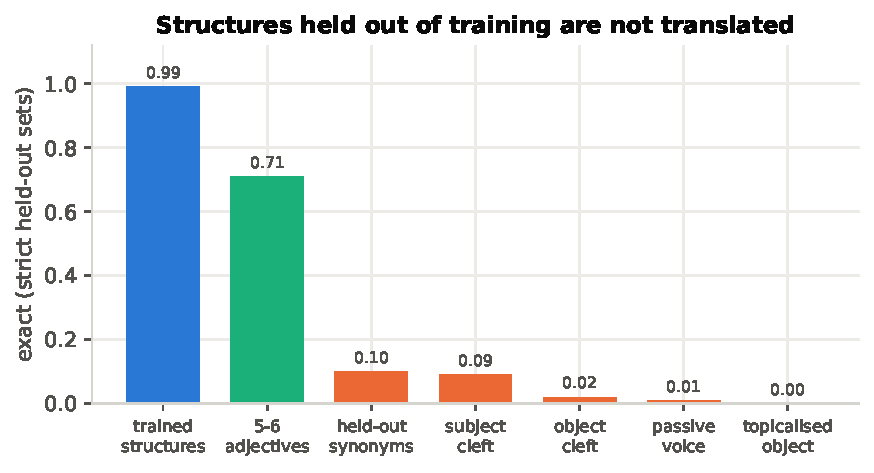
\includegraphics[width=0.53\linewidth]{figures/fig_heldout_structures.pdf}\hfill
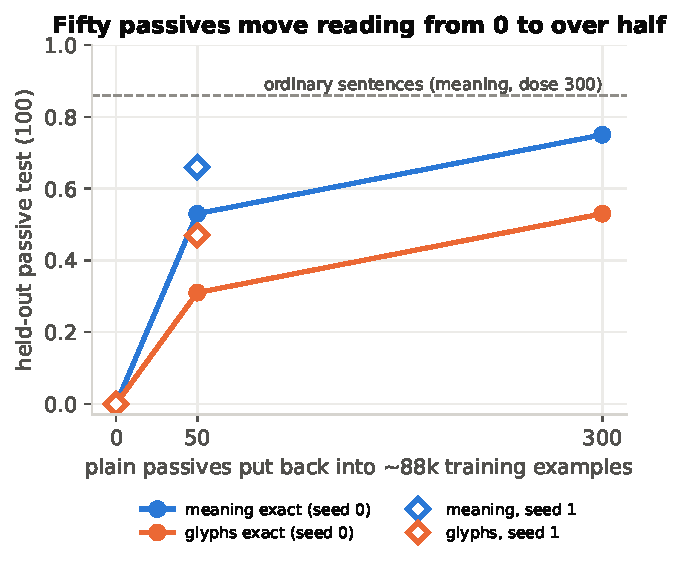
\includegraphics[width=0.44\linewidth]{figures/fig_passive_dose.pdf}
\caption{Left: English structures held out of training (first language version, analysis-first model, 5 epochs;
three runs give 0.00--0.09 on every held-out structure). Right: passives put back as a dose, nothing else changed
(1 run per dose; diamonds: second training seed).}
\label{fig:claimA}
\end{figure}

Holding 20\% of English structure variants out of training gives near-zero accuracy on exactly those structures
(passive 0.00--0.02, clefts 0.01--0.09, topicalised objects 0.00--0.01, three runs) while trained structures stay at
0.97--0.99 (Figure~\ref{fig:claimA}, left). The misreading is by position: a passive takes its first noun as the
doer. A dose test isolates the cause in the final language: with only plain passives held out and 0, 50 or 300 put
back into $\sim$88k examples, held-out passive meaning goes 0.00 / 0.53 / 0.75, and the 0 $\rightarrow$ 50 step
replicates on a second seed (0.00 / 0.66) (Figure~\ref{fig:claimA}, right). Fifty examples, 0.06\% of the data,
switch the structure on; the rest of the language is unchanged.

The same limit appears in arithmetic written in glyph digits (base 7). Removing every training multiplication that
needs one single-digit fact drops problems that need it to 0.05 (5$\times$6), 0.10 (3$\times$4) and 0.41
(2$\times$2), while problems that avoid it stay at 0.91--0.96; a control that also removes the swapped twin keeps
the avoid-group at 0.82--0.89. A bridge run that trains base conversion of every product, including the removed one,
still does not rebuild 5$\times$6 (problems needing it 0.03). A scratchpad trained on workings with at most 3 steps
per row writes exactly 2 rows of 3 steps on every longer problem (1,798 of 1,800 rows; exact 0.00--0.01): it learned
the template of its longest working, not the loop, the subgraph-matching pattern of \citet{dziri2023faith}.

\textbf{Strength: strong} as a description (many runs, two seeds where tested); causal for one structure and one
fact. New relative to prior work: the 50-example dose and the fixed scratchpad shape with dropped-digit answers.
Training much longer does not remove the limit either: with weight decay 1.0 and up to 60k steps we saw no grokking
(no late jump in test accuracy) in translation or maths (Appendix~\ref{app:grok}).

\subsection{B. A spelling rule transfers only when it covers the vocabulary}\label{sec:claimB}

\begin{figure}[t]
\centering
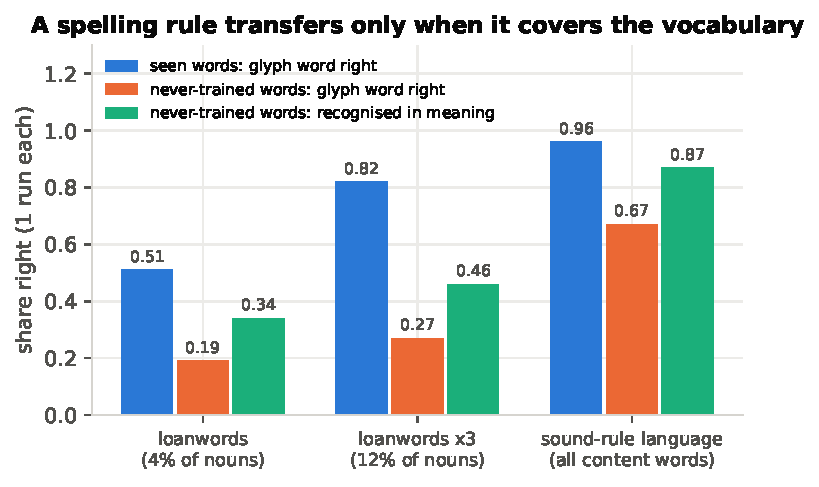
\includegraphics[width=0.62\linewidth]{figures/fig_rule_vs_list.pdf}
\caption{Words spelled by fixed sound rules from their English letters. Loanwords: only a minority of nouns follow
the rule (rate 0.04, and 0.12 in the ``$\times$3'' run). Sound-rule language: every content word does, and 20\% of
content words (2,232) never appear in training. 1 run per condition, 300--600 generated sentences.}
\label{fig:claimB}
\end{figure}

Two extensions spell words by the same letter-to-sound rules (\emph{b}$\rightarrow$\emph{p},
\emph{th}$\rightarrow$\emph{t}, \ldots). If the rule were learned, words never seen in training should be spelled
almost as well as seen ones. When only loanwords follow it (4\% of nouns, marked \an{LOAN}), new loans are spelled
right 0.19 against 0.51 for seen loans; tripling the loan rate lifts seen loans to 0.82 but new loans only to 0.27,
missing the pre-registered +0.10, and the seen--new gap grows from 0.32 to 0.55 (Figure~\ref{fig:claimB}). Some of
the rule is learned: one-letter mappings transfer better than multi-letter ones (0.23 vs 0.12, Fisher $p=0.005$),
and near-miss spellings rise from 21\% to 33\% of errors. Recognition fails first: only 0.34--0.46 of new loans are
marked as loans; most are written as a bare English word the language does not have. When \emph{every} content word
follows the rule, never-trained words are spelled right 0.67 (seen words 0.96 in the same sentences) and recognised
0.87, at no cost elsewhere (generated glyphs 0.71 vs 0.61 baseline).

\textbf{Strength: moderate} (1 run per condition). The two conditions also differ in what must be recognised, and
the general idea is known (Tolerance Principle); we claim only the two ends, not a threshold.

\subsection{C. Only English variety helps real English}\label{sec:claimC}

\begin{figure}[t]
\centering
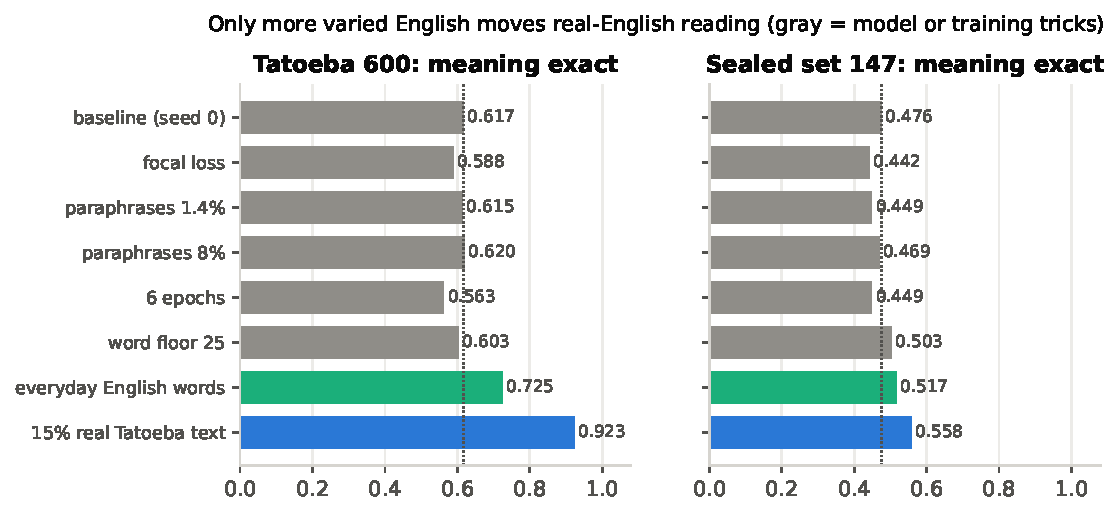
\includegraphics[width=0.86\linewidth]{figures/fig_english_variety.pdf}
\caption{One change per run against the baseline. Gray: model, loss and training-length changes; green: the common
English words and uses the generator left out (no reader labels); blue: 15\% real Tatoeba sentences. Sealed numbers
are totals over 147 sentences.}
\label{fig:claimC}
\end{figure}

Trained models read generated English almost perfectly (0.943 of sentences with every meaning fact right), but real
English is far harder: Tatoeba meaning 0.62, sealed 0.47. Replacing 15\% of training with real Tatoeba sentences
lifts Tatoeba meaning to 0.923 / 0.928 (2 seeds; +0.307, 189 fixes vs 5 breaks, $p=1.8\times10^{-49}$) and sealed
meaning from 0.476 / 0.463 to 0.558 / 0.558 (paired McNemar $p=0.036$ / $0.013$ per seed; not significant after the
Holm correction). Because Tatoeba gold and the real training labels come from the same automatic reader, and the
hand-check finds the gold right in 0.61 of the gained sentences, about +0.19 of the +0.31 rests on correct labels. A
run that adds only the everyday English words and uses the generator never produced (main-verb \emph{have/do},
\emph{people}, \emph{just}, nouns made from verbs; no real sentences, no reader labels) gains +0.11 on Tatoeba
(77 fixes vs 12 breaks, $p<10^{-11}$) and +0.04 on the sealed set (1 run).

Every alternative tried is null or harmful on real English (Figure~\ref{fig:claimC}): focal loss ($-0.028$,
$p=0.014$), paraphrased training English at 1.4\% and 8\% of the data, a word floor of 25, 6 epochs instead of 4
($-0.053$, $p=0.0002$, also after Holm: more epochs fit the generated style), a two-stage rewriter, beam search and
majority voting over samples (changes below 0.01), and Qwen3-1.7B (Tatoeba reading failures 0.37 vs 0.38 at the
same 2 epochs; the pre-registered $\ge$0.05 improvement fails). Of the baseline's 217 never-seen word occurrences on
Tatoeba, most are everyday words and uses, not rare words; real text cuts them to 20.

\textbf{Strength: strong on Tatoeba} (2 seeds), \textbf{moderate on the sealed set}. The synthetic-to-real gap is
known \citep{herzig2019detect}; our contribution is a controlled test against eight alternatives.

\subsection{D. On real English, reading fails; with untrained words, both}\label{sec:claimD}

\begin{figure}[t]
\centering
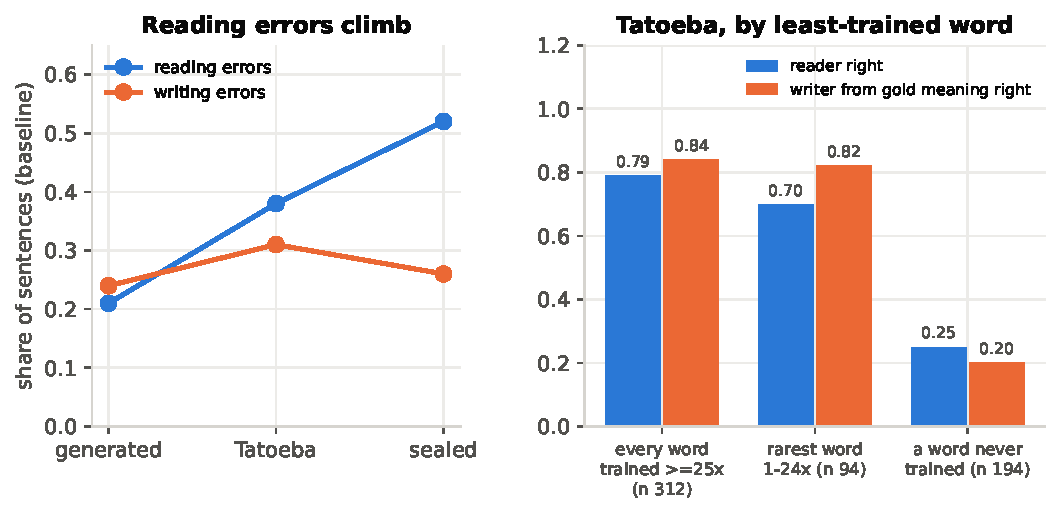
\includegraphics[width=0.88\linewidth]{figures/fig_reading_writing.pdf}
\caption{Left: share of sentences with a reading error ($\hat m\neq m$) and a writing error (judged on the model's
own meaning) for the baseline as the English moves away from training. Right: separate reader and writer models,
the writer given the gold meaning, on Tatoeba by the least-trained word key in the meaning (1 run each).}
\label{fig:claimD}
\end{figure}

Judged on the model's own meaning, the baseline's writing errors stay roughly flat from generated to Tatoeba to sealed
sentences (0.24, 0.31, 0.26) while reading errors climb (0.21, 0.38, 0.52) (Figure~\ref{fig:claimD}, left). On
held-out English structures 73--75\% of items are misread and only 0.4--1.6\% miswritten. To separate the two
causally we trained a reader alone (English $\rightarrow$ meaning) and a writer alone (meaning $\rightarrow$
glyphs). The reader is wrong in 74\% (Tatoeba) and 90\% (sealed) of pipeline failures; on held-out passives the
reader scores 0.00 while the writer, given the gold meaning, writes 0.72. But the writer from gold is right only
0.63 on Tatoeba. A per-sentence test with predictions written beforehand shows why (Figure~\ref{fig:claimD}, right):
the writer is right 0.84 when every word key of the meaning was trained at least 25 times, 0.82 when the rarest was
seen 1--24 times, and 0.20 when one was never trained (a third of Tatoeba); the reader also fails there (0.25). The
sealed set goes the same way (0.93 vs 0.34). For passives the mechanism is in the representation: a linear probe
cannot read the passive doer from the hidden states of the model trained without passives beyond what the surface
words give (0.746 vs 0.704), but reads it in models trained on passives (0.871, 0.950).

\begin{figure}[t]
\centering
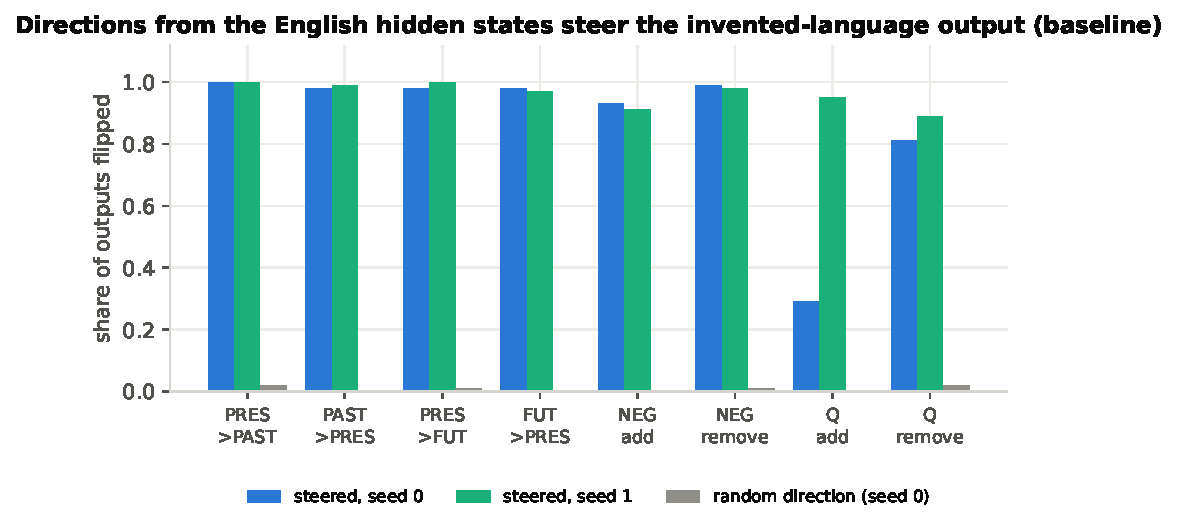
\includegraphics[width=0.80\linewidth]{figures/fig_steering.pdf}
\caption{Steering the baseline: a mean-difference direction (from English hidden states of sentences with the two
values) is added at layer 6 while the model reads the English. Flip: the output's meaning now carries the target
value. Random: a same-size random direction. 100 generated sentences per pair.}
\label{fig:steer}
\end{figure}

\paragraph{Inside the model:} Why does reading, rather than writing, fail? Linear probes read tense, negation,
question, aspect, modality and subject from the hidden states of every model at 0.90--1.00. Steering shows that the
output is written from this English-side representation: adding the tense direction flips the output tense in
0.97--1.00 of sentences and negation in 0.91--0.99, against $\le$0.02 for random directions, on four models (two
training seeds each of the baseline and the real-text model; Figure~\ref{fig:steer}), and subject pushes repair 11 of
12 and 10 of 10 real Tatoeba subject errors (random or shuffled-label pushes repair at most 3). Where the output is wrong
on Tatoeba, the probe is usually wrong too (right 0.41, below the majority-class rate 0.79) and in 59\% of cases reads
the same wrong value the output wrote: most real-English errors are already in the English representation, and the
writer faithfully renders them. Tense steering itself is known \citep{klerings2025tense}; here it serves as evidence
for where the errors sit.

\textbf{Strength: moderate} (1 run per model for the reader/writer split, 2 seeds for probes and steering; the split
was examined after the first results, and the later predictions were written before their runs). The usual low-resource finding is the opposite
\citep{bafna2025barrier}; here the target language is dense in training and the English input is the unfamiliar
side.

\subsection{E. In maths, a missing fact is rebuilt only from facts seen in the same role}\label{sec:claimE}

\begin{figure}[t]
\centering
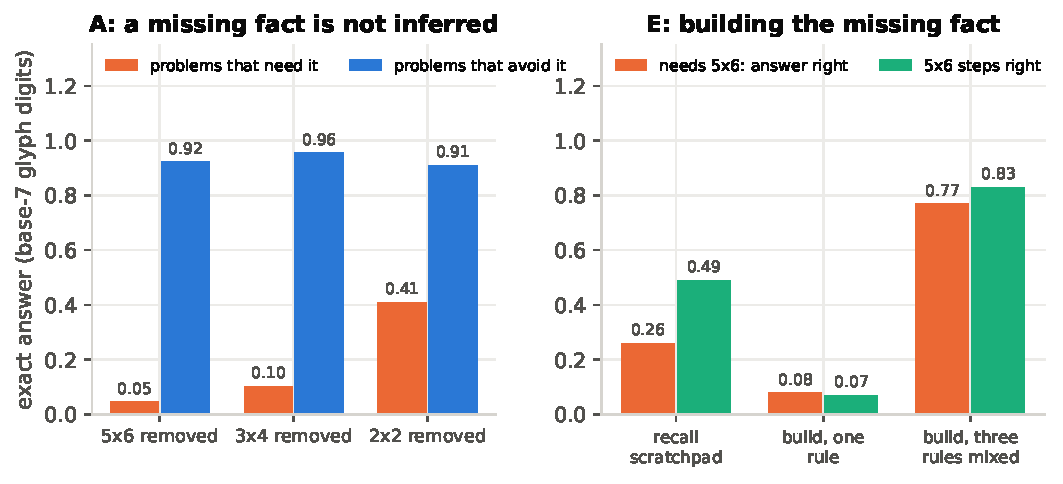
\includegraphics[width=0.84\linewidth]{figures/fig_maths.pdf}
\caption{Arithmetic in base-7 glyph digits. Left: removing every training problem that needs one fact (claim A).
Right: three scratchpads with 5$\times$6 and 6$\times$5 removed from training.}
\label{fig:maths}
\end{figure}

Claim A showed that a model trained without 5$\times$6 cannot infer it. We then asked what it takes to make it
\emph{build} the missing fact, in four steps (all with 5$\times$6 and 6$\times$5 absent from training, checked).

\emph{1. Recall the facts in a scratchpad} (\an{5x6+0=42}): every other step of the working is right (857 of 857),
but the written 5$\times$6 steps are right only 0.49, and problems needing them 0.26 (Figure~\ref{fig:maths}, right).
The model guesses: the same problem gets the same 5$\times$6 value only 60\% of the time, and a vote over 8 sampled
workings does not help (0.27).

\emph{2. Build each product from a smaller one, with one rule} (\an{5x6=5x4=26+5=34+5=42}): the model follows the
procedure and adds correctly, but problems needing 5$\times$6 drop to 0.08. It writes the block wrong
(\an{5x6=5x4=22+\ldots}) although it computes 5$\times$4 = 26 correctly as an ordinary step: with one rule,
5$\times$4 appeared \emph{as a building block} only inside the removed 5$\times$6 working.

\emph{3. Mix three building rules}, so the same facts also appear as blocks in other workings: problems needing
5$\times$6 rise to 0.77 and its steps to 0.83. Of the 5$\times$6 steps, 80\% are built from a block seen in that role
(5$\times$4, 6$\times$3, 6$\times$4), and these are right 99.6\% of the time; the other 20\% use a block never seen
in that role (4$\times$6, 5$\times$5) and are right 17\%. The same recipe rebuilds other removed facts: 5$\times$6
on a second seed 0.72, 3$\times$4 0.98, 6$\times$6 0.64 (Figure~\ref{fig:role}, right); with the whole large end of
the 6 row removed it recovers 0.57--0.72 of four facts and 0.00 of 6$\times$5. Forcing every possible route on every
problem, 15 of 18 blocks follow the rule (seen as a block: right; never seen as a block: wrong), and a failing route
writes a neighbour's value in the block slot (the 5$\times$5 slot gets 26, the value of 5$\times$4).

\emph{4. How many examples of the role are needed?} Keeping one building rule, 5$\times$4 is shown as a block in
$N$ training workings. The written 5$\times$6 steps are right 0.00 / 0.91 / 1.00 / 0.96 / 0.93 at $N$ = 0 / 5 / 25
/ 100 / 400 (Figure~\ref{fig:role}, left): the curve is a step, not a slope, and five examples are enough. The dose
never reaches the other order: 6$\times$5, built from a block the dose does not touch, stays at 0.06 even at the
largest dose (593 workings). Order alone is different: with only 6$\times$5 removed and 5$\times$6 still in
training, the plain recall scratchpad writes the never-seen 6$\times$5 step right in 172 of 174 cases.

\begin{figure}[t]
\centering
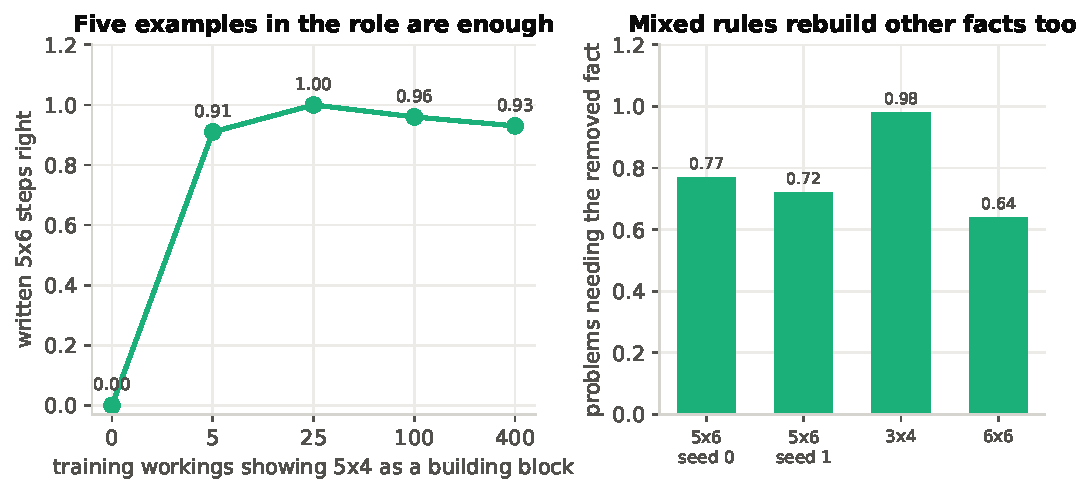
\includegraphics[width=0.80\linewidth]{figures/fig_maths_role.pdf}
\caption{Left: one building rule, with 5$\times$4 shown as a building block in $N$ training workings. Right: the
mixed-rule scratchpad with other facts removed and a second seed.}
\label{fig:role}
\end{figure}

So the model can compute a fact it never saw, but only by recombining facts it has already used \emph{in the same
role}; a fact it knows only in another role is not reused, which links coverage (claim A) to how facts are stored.
Caveat: each condition is one training run, and same-seed maths runs vary by about $\pm$0.1--0.2 (GPU
non-determinism), so single values are approximate; the second seed is less clean (seen-role blocks 0.84, never-seen
0.56).

%=====================================================================
\section{Limitations}\label{sec:limitations}

\begin{itemize}
\item \textbf{Run counts.} Most extension results are single training runs; real text, steering and the passive
0/50 dose have two seeds. On the 147-sentence sealed set only differences above about 0.11 are clear for a single
comparison, and the Tatoeba gold is the automatic reader's (about a third wrong by a 70-sentence hand-check).
\item \textbf{GPU non-determinism.} Same-seed maths re-runs with byte-identical data differ by $\pm$0.1--0.2 on the
needs-pair tests (non-deterministic attention backward pass). A \texttt{--deterministic} option makes full language
runs reproduce exactly on two different machines; all maths numbers are single draws.
\item \textbf{One model family and size} (Qwen3-0.6B, one 1.7B run) and one invented grammar; claims B and D were
partly formed after the first data, and are marked as such.
\item \textbf{Sealed set.} Its gold meanings are reader output with hand corrections, so a model trained on reader
labels can partly gain by learning reader conventions; the everyday-words run, which uses no reader labels, is the
cleaner evidence for claim C.
\end{itemize}

%=====================================================================
\section{Future work}\label{sec:future}

The following extend experiments that already have results; their predictions are written but they were not run
for this report.
\begin{itemize}
\item \textbf{Seed replicates for claim B}: a second training seed of the sound-rule language (does 0.67 for
never-trained words replicate?).
\item \textbf{Intermediate rule coverage for claim B}: languages in which 25\% and 50\% of content words are
rule-spelled, to see whether the change between a 4--12\% minority (0.19--0.27) and the whole vocabulary (0.67) is
gradual or sharp, as \citet{friedman2026tolerance} would predict for gradual.
\item \textbf{Three deterministic seeds for claim E}: the mixed-rule scratchpads (5$\times$6, 3$\times$4,
6$\times$6, whole 6 row removed) and the 0- and 5-workings role doses, each with three seeds, judged on 3-seed means
against the written thresholds (seen-role blocks $\ge$0.90, never-seen-role blocks $\le$0.30).
\item \textbf{Determinism for maths}: confirming that the attention fix makes maths runs bit-identical, so that
single-run thresholds in claims A and E can be re-judged without seed noise.
\end{itemize}

%=====================================================================
\section{Conclusion}

A small model learns an invented language with its own script well, but it generalises only as far as its training
covers: unseen structures fail and fifty examples switch one on; a spelling rule transfers when it covers the
vocabulary and stays a list when it covers a minority. On real English the limit is reading the English, not
writing the new language, and only more varied English in the training data moves it; loss functions, decoding,
more epochs and a 3$\times$ larger model do not. Inside the model, the invented-language output is driven by the
model's English meaning representation, and most real-English errors are already present there. In arithmetic, a
missing fact can be rebuilt, but only from facts seen in the same role. For anyone adapting a small model to a new language, the practical lesson is to spend effort on
the coverage and variety of the source-language side of the data.

\subsubsection*{Acknowledgments}
Compute: free Kaggle GPUs (three accounts, two lent by friends), a laptop RTX 2050, and one paid cloud session of
about USD 1.60. Concept images in the presentation are credited in Appendix~\ref{app:credits}.

\bibliography{references}
\bibliographystyle{iclr2025_conference}

%=====================================================================
\newpage
\appendix

\section{The invented language}\label{app:language}

\paragraph{Grammar:} Subject--object--verb order, no articles, case endings (object, location and 21 relation cases
such as ON, TO, WITH, FROM), every tense an ending, full person/number/gender agreement on the verb, a negation
ending, irregular past stems, progressive, perfect and modal endings (CAN, MUST, SHOULD, MAY, WOULD, LET), yes/no
questions as an ending, question words left in place, and sound changes (sandhi) where pieces join.

\paragraph{Vocabulary:} 11,078 root words (including 2,355 abstract and mass nouns), hand-listed everyday words, and
words built from stackable pieces: \an{fun>ADJ} (funny), \an{hope>LESS} (hopeless), \an{run>AGENT} (runner),
\an{happy>NOT>QUAL} (unhappiness); 2,127 such words verified with WordNet, plus compounds such as \an{book\_shop}.

\paragraph{Script:} 27 invented glyphs from the Unicode Private Use Area, an abugida like Tamil script (each sign a
consonant with an inherent vowel, or a vowel). Without being added to the vocabulary each glyph would be split into
three byte tokens; we add each as one new token.

\paragraph{Analysis fields:} Each event has optional fields \an{S} (doer), \an{V} (verb with endings), \an{O}
(object), \an{L} (place), \an{M} (manner), \an{A} (describing words after ``be''), \an{P} (noun after ``be''),
\an{C} (joining word), \an{I} (greeting), \an{Y} (person spoken to), \an{T} (time phrase) and one field per relation
(\an{ON=}, \an{TO=}, \ldots); events are separated by ``;''. Partial inputs (a bare noun phrase, a bare verb) are
also translated.

\paragraph{Earlier version:} The first language version (4,320 English content words, one event per sentence) was
used for the held-out structure study (Figure~\ref{fig:claimA}, left) and the script study (Appendix~\ref{app:script}).
The final version keeps every first-version form unchanged (checked on 4,587 clauses).

\section{Training details and compute}\label{app:training}

\begin{center}\small
\begin{tabular}{lp{0.72\linewidth}}
\toprule
Base model & Qwen3-0.6B-Base (one run: Qwen3-1.7B-Base, 2 epochs) \\
Adapter & LoRA $r=16$, $\alpha=32$, dropout 0; q, k, v, o, gate, up, down projections \\
New tokens & 27 glyphs, trainable tied embeddings, start = embedding of the glyph's sound \\
Optimiser & AdamW, lr $2\times10^{-4}$, weight decay 0, 3\% warm-up, linear decay \\
Batch & 16 $\times$ 2 gradient accumulation; long batches split by a 1,600-token budget \\
Data & 80,000 translation + 2,500 refusal + 6,000 replay examples; word floor 12 \\
Length & 4 epochs, 11,064 steps; fp16; about 6 GPU-hours on a Kaggle T4 \\
Compute & free Kaggle (about 30 GPU-h per account per week), laptop RTX 2050 (4 GB) for scoring, probes, steering \\
\bottomrule
\end{tabular}
\end{center}

\section{Stage 1: the script and the tokenizer}\label{app:script}

The project began with a tokenization question: does the number of tokens a script costs predict how well a model
learns a language written in it? In a 2$\times$2 grid (English-like vs Tamil-like grammar, Latin vs Tamil script,
three random languages per cell, 20k sentences) content-word accuracy was 0.82 (easy, Latin), 0.86 (easy, Tamil
script, 3$\times$ more tokens), 0.04 (hard, Latin) and 0.24 (hard, Tamil script): more tokens did not mean worse
learning, and grammar dominated; at 50k sentences all four cells reach 0.98--0.99. What hurt was \emph{byte pieces
that do not line up with known characters}: invented glyphs split into 3 byte tokens collapse at 20k sentences
(exact 0.00). Adding each glyph as one token, with its embedding starting at the embedding of its sound, is
the method used in all main runs.

\begin{figure}[h]
\centering
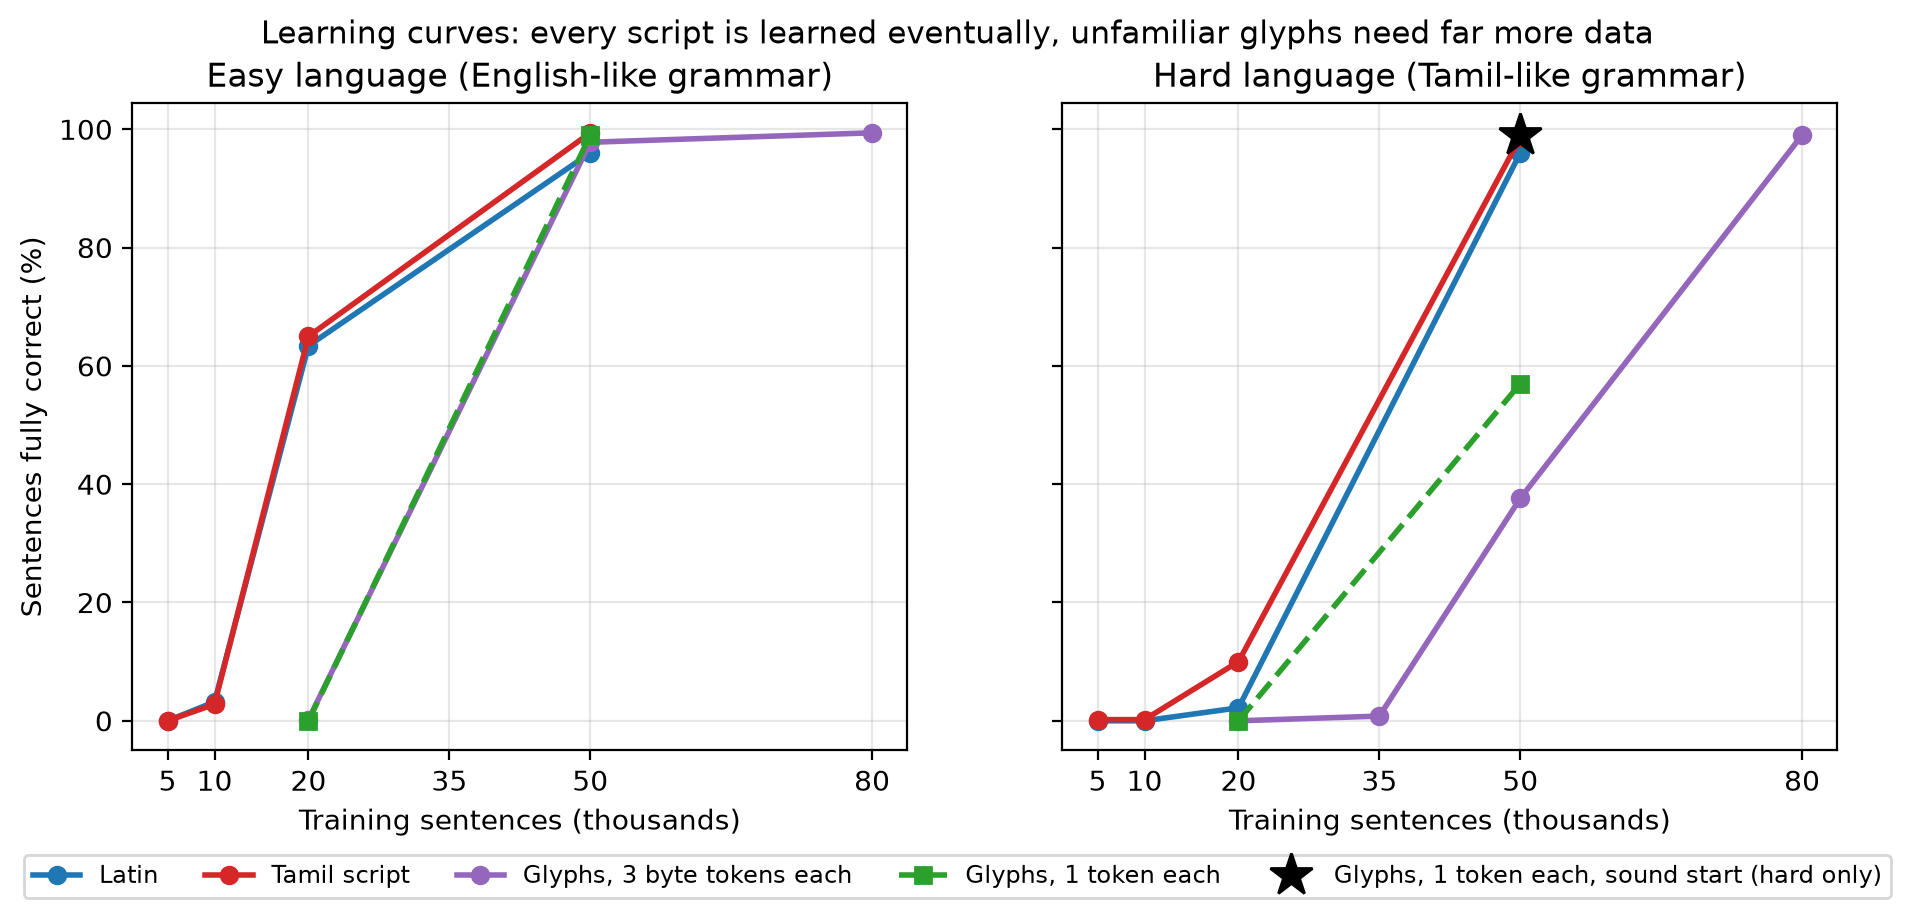
\includegraphics[width=0.62\linewidth]{figures/fig1_learning_curves.png}
\caption{Stage 1 learning curves: content-word accuracy against training sentences for the four grammar $\times$
script cells and the invented-glyph runs (first language version).}
\end{figure}

\section{Additional results}\label{app:more}

\begin{figure}[h]
\centering
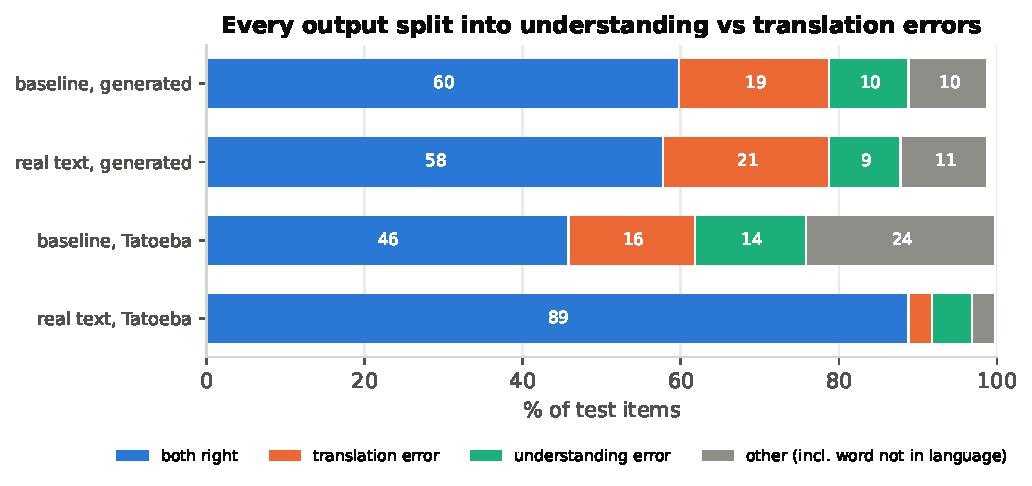
\includegraphics[width=0.74\linewidth]{figures/fig_error_split.pdf}
\caption{Every output classified by comparing the analysis and the glyphs with the gold (\% of items, 1 seed each).
``Other'' is mostly an analysis using a word the language does not have. Real text removes most errors on Tatoeba
but none of the translation errors on generated sentences: what it adds is vocabulary, not a better command of the
endings.}
\end{figure}

\paragraph{Decoding:} On Tatoeba, beam search with 4 beams gives meaning exact 0.618 vs 0.617 greedy (5 fixes, 4
breaks, $p=1.0$) and a majority vote of 5 samples 0.622 ($p=0.51$): other outputs repeat the same misreading.

\paragraph{What the base model knows:} On generated statements the untrained base model answering comprehension
questions gets 0.649 of facts right, the instruct version 0.725, and linear probes on the frozen base model recover
tense 0.94--0.99, negation 0.99--1.00 and word role 0.87--0.89. The fine-tuned baseline reaches 0.987: the base model
encodes much more than it can be prompted to say.

\paragraph{Real English by epoch:} The baseline's meaning on Tatoeba is 0.577 / 0.612 / 0.617 after epochs 1 / 2 / 4
and on the sealed set 0.429 / 0.463 / 0.476: reading real English is almost settled by epoch 2; later epochs mainly
improve the glyphs.

\paragraph{Why the sealed set is harder than Tatoeba:} An automatic totals-only breakdown (predictions written first)
finds that on single-clause sentences the baseline scores the same on the sealed set as on Tatoeba (0.61 vs 0.62);
the gap comes from multi-clause sentences (sealed 0.17), which are a third of free writing but 1\% of Tatoeba.
Real text adds +0.15 on single clauses and nothing on multi-clause ones.

\section{Side study: no grokking}\label{app:grok}

Grokking is a late jump in test accuracy long after training accuracy saturates, usually seen with strong weight
decay on small algorithmic datasets \citep{power2022grokking}. If it happened here, held-out combinations might be
learned with enough training instead of more data. We trained three small settings far past saturation with weight
decay 1.0 (on the LoRA adapter and the new embeddings; the base model is frozen):

\begin{center}\small
\resizebox{\linewidth}{!}{\begin{tabular}{lccccc}
\toprule
Run & Steps & Train & Test (end) & Extra test (end) & Logit norm \\
\midrule
translation, 4,000 sentences & 12,000 & 0.93 & 0.80 (new combinations) & 0.49 (new clause structure) & 1,570 $\rightarrow$ 3,130 \\
maths, 40\% of the table & 60,000 & 1.00 & 0.73 (new pairs) & 0.11 (3-digit) & 1,160 $\rightarrow$ 5,720 \\
maths, 60\% of the table & 60,000 & 0.99 & 0.84 (new pairs) & 0.09 (3-digit) & 4,599 $\rightarrow$ 5,603 \\
\bottomrule
\end{tabular}}
\end{center}

\begin{figure}[h]
\centering
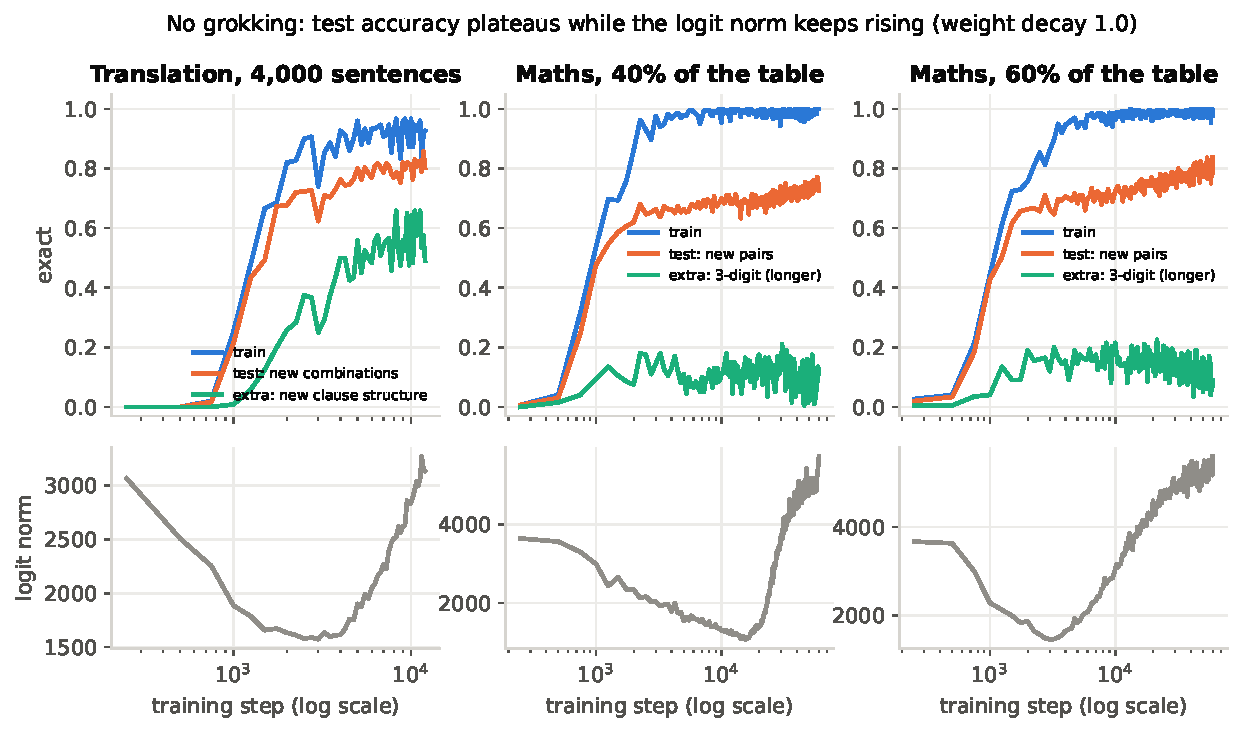
\includegraphics[width=\linewidth]{figures/fig_grokking.pdf}
\caption{Training curves of the three grokking runs (log step axis). Top: train, test and harder ``extra'' test
accuracy. Bottom: the norm of the output logits.}
\label{fig:grok}
\end{figure}

There is no grokking transition in any of the three (Figure~\ref{fig:grok}). Training accuracy saturates around
step 6,000; the translation test is flat from about 4k steps and the 40\% maths test stays at 0.71--0.76 from about
6k. With 60\% of the table the test score keeps rising slowly (0.74 at 20k steps to 0.84 at 60k), so a later gradual
improvement cannot be ruled out, but there is no jump, and the longer 3-digit problems never improve. The logit norm
first falls and then rises steadily: the model makes its memorised answers more confident instead of simplifying,
the opposite of the grokking signature. Caveat: the 40\% run used weight decay 0.1 for its first 16k steps (resumed
from a checkpoint), so 40\% vs 60\% is not a clean comparison.

\section{Code}\label{app:code}

The code is submitted with this report and is public at
\url{https://github.com/Lsidvd234/alien-rosetta}. Main parts: \texttt{conlang/} (grammar, lexicon, script and the v2
generator), \texttt{train/run.py} (data building, glyph tokens and their initialisation, LoRA training, evaluation),
\texttt{train/maths.py} (base-7 arithmetic and scratchpads), \texttt{analysis/} (scoring, significance tests, error
split, reader/writer bottleneck, loanword and sound-rule analysis, probes and steering), \texttt{kaggle\_tools/}
(job queues for free Kaggle GPUs), and \texttt{sealed/} (the frozen test set is not included).

\section{Image credits (presentation)}\label{app:credits}
Tamil alphabet chart: public domain,
Wikimedia Commons. Decoder-only transformer diagram: Marxav, CC BY-SA 4.0, Wikimedia Commons. LoRA diagram: Figure 1
of \citet{hu2022lora}. Activation-addition diagram: Figure 1 of \citet{turner2023actadd}.

\end{document}
